%This template is created by SV Bùi Vân Anh, và Thầy Nguyễn Tiến Hòa từ phòng Lab xử lý tín hiệu băng gốc hệ thống 5G.
%%%%%%%%%%%%%%%%%%%%%%%%%%%%%%%%%%%%%%%%%%%%%%%%%%%%%%%
\documentclass{article}
\usepackage{amsmath}
\usepackage{algorithm}
\usepackage{algpseudocode}
\usepackage{amsfonts}
\usepackage{multirow}
\usepackage[utf8]{inputenc}
\usepackage[english,vietnamese]{babel}
\usepackage{ragged2e}
\selectlanguage{vietnamese}
\usepackage[style=ddmmyyyy]{datetime2}
\DTMlangsetup[vi]{ord=raise}
\usepackage[T5]{fontenc}
\usepackage[fontsize=13pt]{scrextend}
\usepackage[paperheight=29.7cm,paperwidth=21cm,right=2cm,left=3cm,top=2cm,bottom=2.5cm]{geometry}
\usepackage{pgfplots}
\pgfplotsset{compat=1.18}
\usepackage{enumitem}
\setlist[itemize]{leftmargin=1cm}
\usepackage{mathptmx}
\usepackage{graphicx}
\usepackage{float}
\usepackage{subcaption}
\usepackage{tikz}
\usetikzlibrary{calc, shapes.geometric}
\usepackage{indentfirst}
\usepackage{booktabs}
\renewcommand{\baselinestretch}{1.2}
\setlength{\parskip}{6pt}
\setlength{\parindent}{1cm}
\usepackage{titlesec}
\setcounter{secnumdepth}{4}
\titlespacing*{\section}{0pt}{0pt}{30pt}
\titleformat*{\section}{\fontsize{16pt}{0pt}\selectfont \bfseries \centering}
\titlespacing*{\subsection}{0pt}{0pt}{0pt}
\titleformat*{\subsection}{\fontsize{14pt}{0pt}\selectfont \bfseries}
\titlespacing*{\subsubsection}{0pt}{10pt}{0pt}
\titleformat*{\subsubsection}{\fontsize{13pt}{0pt}\selectfont \bfseries }
\titlespacing*{\paragraph}{0pt}{10pt}{0pt}
\titleformat*{\paragraph}{\fontsize{13pt}{0pt}\selectfont\bfseries }

\renewcommand{\figurename}{\fontsize{12pt}{0pt}\selectfont \bfseries Hình}
\renewcommand{\thefigure}{\thesection.\arabic{figure}}
\usepackage[font=bf]{caption}
\captionsetup[figure]{labelsep=space}

\renewcommand{\tablename}{\fontsize{12pt}{0pt}\selectfont \bfseries Bảng}
\renewcommand{\thetable}{\thesection.\arabic{table}}
\captionsetup[table]{labelsep=space}

\usepackage{tabularx}
\newcolumntype{s}{>{\hsize=.3\hsize}X}
\newcolumntype{y}{>{\hsize=.4\hsize}X}
\newcolumntype{d}{>{\hsize=.1\hsize}X}
\newcolumntype{a}{>{\hsize=1.1\hsize}X}
\newcolumntype{g}{>{\hsize=5\hsize}X}
\renewcommand{\tabularxcolumn}[1]{>{\small\arraybackslash}p{#1}}

\renewcommand{\theequation}{\thesection.\arabic{equation}}
\newtheorem{theorem}{Định lý}[section]
\newtheorem{defn}[theorem]{Định nghĩa}
\newtheorem{corollary}[theorem]{Hệ quả}
\newtheorem{lemma}[theorem]{Bổ đề}

\usepackage{lipsum}
\renewcommand{\contentsname}{MỤC LỤC}
\renewcommand{\listfigurename}{DANH MỤC HÌNH VẼ}
\renewcommand{\listtablename}{DANH MỤC BẢNG BIỂU}
\renewcommand{\refname}{TÀI LIỆU THAM KHẢO}
\usepackage[unicode]{hyperref}
% Removed colortbl
\usepackage{forloop}
\newcounter{loopcntr}
\newcommand{\rpt}[2][1]{\forloop{loopcntr}{0}{\value{loopcntr}<#1}{#2}}

% ==========================================
% TRANG BÌA VÀ THÔNG TIN BÁO CÁO
% ==========================================
\title{\textbf{BÁO CÁO DỰ ÁN}\\ \Large HỆ THỐNG NHÚNG CHUẨN HÓA KẾT NỐI & QUẢN LÝ ĐA CẢM BIẾN}
\author{Nhóm phát triển}
\date{\today}

\begin{document}

% 1. Trang bìa
\begin{titlepage}
\begin{tikzpicture}[overlay,remember picture]
\draw[line width=3pt]
    ($ (current page.north west) + (1.2cm,-1.5cm) $) 
    rectangle
    ($ (current page.south east) + (-1.1cm,1.5cm) $); 
\draw[line width=0.5pt]
    ($ (current page.north west) + (1.1cm,-1.4cm) $) 
    rectangle
    ($ (current page.south east) + (-1.0cm,1.4cm) $);
\end{tikzpicture}
\begin{center}
\vspace{-12pt}   ĐẠI HỌC BÁCH KHOA HÀ NỘI \\
\textbf{\fontsize{16pt}{0pt}\selectfont TRƯỜNG ĐIỆN - ĐIỆN TỬ}
\vspace{0.5cm}
 \begin{figure}[H]
     \centering
     
\includegraphics[width=3cm,height=4cm]{pic/logodhbk.png}
     \vspace{1cm} % Giữ chỗ cho logo
 \end{figure}
\vspace{0.5cm}\href{}{}
\fontsize{24pt}{0pt}\selectfont BÁO CÁO\\
\vspace{12pt}
\textbf{\fontsize{32pt}{0pt}\selectfont BÀI TẬP LỚN MÔN HỌC LẬP TRÌNH WEB VÀ ỨNG DỤNG}
\vspace{1cm}
\end{center}
\hspace{6pt}\textbf{\fontsize{14pt}{0pt}\selectfont Đề tài:}
\begin{center}
    \textbf{\fontsize{20pt}{0pt}\selectfont HỆ THỐNG NHÚNG CHUẨN HÓA KẾT NỐI \& QUẢN LÝ ĐA CẢM BIẾN}\\

\vspace{0.5cm}
\begin{table}[H]
    \centering
    \begin{tabular}{l l}
 \fontsize{14pt}{0pt}\selectfont Sinh viên thực hiện:    & \fontsize{14pt}{0pt}\selectfont HỒ QUANG QUÂN - 20241848E\vspace{6pt} 
                                                            \\ &\fontsize{14pt}{0pt}\selectfont HỒ XUÂN PHÚ - 20250179E  \vspace{6pt}\\

\fontsize{14pt}{0pt}\selectfont Giảng viên hướng dẫn: & \fontsize{14pt}{0pt}\selectfont TS.NGUYỄN THANH TÙNG
\end{tabular}
\end{table}
\vspace{1cm}
 \fontsize{14pt}{0pt}\selectfont Hà Nội, \today
\end{center}
\end{titlepage}
\cleardoublepage

\thispagestyle{empty}
\newpage

\vspace*{2cm}
\begin{center}
    \fontsize{18pt}{24pt}\selectfont \textbf{TÓM TẮT DỰ ÁN}
\end{center}
\vspace{1cm}
\noindent Dự án "Hệ thống Giám sát Cảm biến Mạng Mesh" đề xuất và triển khai một giải pháp toàn diện cho việc thu thập, giám sát và quản lý dữ liệu môi trường (nhiệt độ, độ ẩm) theo thời gian thực. Bằng cách kết hợp sức mạnh của mạng lưới không dây (Mesh Network) với nền tảng phần mềm hiện đại (React Native, Hệ thống Backend), hệ thống mang lại khả năng mở rộng linh hoạt mà không phụ thuộc vào hạ tầng mạng truyền thống. Điểm nhấn kỹ thuật của dự án bao gồm giao thức truyền thông độ trễ thấp qua WebSocket, hệ thống cảnh báo tự động, và khả năng cập nhật phần mềm từ xa (OTA) cho hàng loạt thiết bị. Báo cáo này trình bày chi tiết từ cơ sở lý thuyết, kiến trúc hệ thống đến các kết quả triển khai thực tế.
\thispagestyle{empty}
\newpage

% Tạo mục lục tự động
\addtocontents{toc}{\protect\thispagestyle{empty}}
\tableofcontents 
\thispagestyle{empty}
\cleardoublepage

\newpage

% Nếu có danh mục hình vẽ
{\let\oldnumberline\numberline
\renewcommand{\numberline}{Hình~\oldnumberline}
\listoffigures} 
\phantomsection\addcontentsline{toc}{section}{\numberline {} DANH MỤC HÌNH VẼ}
\newpage

% Nếu có danh mục bảng biểu
{\let\oldnumberline\numberline
\renewcommand{\numberline}{Bảng~\oldnumberline}
\listoftables}
\phantomsection\addcontentsline{toc}{section}{\numberline {} DANH MỤC BẢNG BIỂU}
\newpage

% ==========================================
% NỘI DUNG CHÍNH CỦA BÁO CÁO
% ==========================================

\section*{CHƯƠNG 1. GIỚI THIỆU VÀ TỔNG QUAN}
\addcontentsline{toc}{section}{\numberline{}CHƯƠNG 1. GIỚI THIỆU VÀ TỔNG QUAN}
\setcounter{section}{1}
\setcounter{subsection}{0}

\subsection{Đặt vấn đề \& Mục tiêu}
Trong kỷ nguyên của Internet vạn vật (IoT), nhu cầu giám sát môi trường và thu thập dữ liệu tự động từ các khu vực rộng lớn ngày càng trở nên cấp thiết. Dự án "Hệ thống Giám sát Cảm biến Mạng Mesh" được đề xuất nhằm xây dựng một nền tảng toàn diện từ phần cứng đến phần mềm, hỗ trợ quản trị viên dễ dàng theo dõi và điều khiển mạng lưới thiết bị theo thời gian thực (Real-time). Mục tiêu chính là xây dựng một ứng dụng đa nền tảng kết nối với trạm trung tâm (Gateway) qua giao thức WebSocket, cho phép giám sát dữ liệu, quản lý lịch sử và cập nhật phần mềm thiết bị từ xa (FOTA).


\subsection{Công nghệ ứng dụng}
\textbf{Frontend (Mobile App):}
\begin{itemize}
    \item \textbf{React Native \& Expo:} Xây dựng giao diện UI mượt mà, đa nền tảng.
    \item \textbf{Zustand:} Quản lý State toàn cục siêu nhẹ, tối ưu re-render thông qua cơ chế hợp nhất (merge) dữ liệu Live liên tục mà không bị mất mát.
    \item \textbf{Expo FileSystem \& Sharing:} Tạo, trích xuất và chia sẻ file báo cáo dữ liệu (CSV) hoàn toàn cục bộ (offline) trên thiết bị.
    \item TailwindCSS / Reanimated để thiết kế hiệu ứng Glassmorphism và các thông báo nổi (Toast Notification) trượt mượt mà.
\end{itemize}
\textbf{Backend Services:}
\begin{itemize}
    \item \textbf{WebSockets:} Kết nối hai chiều (Point-to-Point) để nhận stream dữ liệu Sensor và cập nhật trạng thái thiết bị theo thời gian thực.
    \item \textbf{HTTP API (REST):} Cơ chế truy vấn (GET) để lấy dữ liệu quá khứ từ máy chủ (Server) phục vụ chức năng lịch sử.
    \item \textbf{Nginx Reverse Proxy:} Cấu hình định tuyến và cung cấp chứng chỉ SSL/TLS, cho phép chạy song song giao thức an toàn HTTPS và WSS trên cùng một máy chủ (Port 443).
\end{itemize}

\subsection{Bảng tổng kết chức năng và phân công công việc}
\begin{table}[H]
    \centering
    \renewcommand{\arraystretch}{1.3}
    \begin{tabularx}{\textwidth}{|l|>{\raggedright\arraybackslash}p{2.8cm}|X|>{\raggedright\arraybackslash}p{2.8cm}|}
        \hline
        \textbf{Menu/Phần} & \textbf{Chức năng} & \textbf{Mô tả chi tiết} & \textbf{Phụ trách} \\
        \hline
        Dashboard & Thống kê tổng quan & Hiển thị tóm tắt tình trạng kết nối mạng Mesh và thông số nổi bật nhất của hệ thống. & H. Xuân Phú \\
        \hline
        Nodes & Quản lý thiết bị & Liệt kê danh sách Node, theo dõi trạng thái Online/Offline trực tiếp và cảnh báo mất kết nối. & H. Quang Quân \\
        \hline
        Sensors & Giám sát Realtime & Biểu đồ trực quan và danh sách thông số cảm biến môi trường cập nhật theo thời gian thực. & H. Quang Quân \\
        \hline
        Server & Monitor Backend & Giám sát tài nguyên máy chủ (CPU, RAM, Uptime) và trạng thái hệ thống WebSocket. & H. Xuân Phú \\
        \hline
        Gateway & Monitor Gateway & Giám sát tài nguyên phần cứng (CPU, RAM, Pin, Wi-Fi) và trạng thái của trạm trung tâm. & H. Quang Quân \\
        \hline
        \multirow{2}{*}{History} & Truy vấn quá khứ & Lọc dữ liệu theo mốc thời gian, loại cảm biến, và vẽ biểu đồ lịch sử qua REST API. & H. Xuân Phú \\ \cline{2-4}
        & Trích xuất CSV & Xử lý dữ liệu và tạo file báo cáo CSV cục bộ trên điện thoại để chia sẻ. & H. Xuân Phú \\
        \hline
        Settings & Thiết lập Threshold & Tùy chỉnh các ngưỡng giới hạn (min/max) cảnh báo cho các thông số cảm biến. & H. Quang Quân \\
        \hline
        About & Thông tin \& Hướng dẫn & Tích hợp hướng dẫn sử dụng chi tiết và hiển thị thông tin, tiến độ hoàn thành dự án của nhóm. & H. Quang Quân \\
        \hline
        Backend & Hạ tầng \& Máy chủ & Xây dựng HTTP REST API, cấu hình luồng truyền phát WebSockets và thiết lập Nginx Reverse Proxy trên máy chủ thực tế. & H. Xuân Phú \\
        \hline
        Báo cáo & Tài liệu \& Slide & Soạn thảo báo cáo đồ án và slide thuyết trình tổng kết. & H. Xuân Phú, \par H. Quang Quân \\
        \hline
    \end{tabularx}
    \caption{Bảng phân rã chức năng hệ thống}
\end{table}

\subsection{Bảng tổng kết làm được/chưa làm được}
\begin{table}[H]
    \centering
    \renewcommand{\arraystretch}{1.4}
    \begin{tabularx}{\textwidth}{|X|X|X|}
        \hline
        \textbf{Đã làm được} & \textbf{Điểm mới / Nổi bật} & \textbf{Chưa làm được / Hạn chế} \\
        \hline
        - Xây dựng hoàn chỉnh App React Native đa nền tảng (iOS/Android) tích hợp truyền phát Realtime qua WebSockets. \par
        - Quản lý trạng thái hoạt động của Node/Gateway (Online/Offline) và thông số cảm biến theo thời gian thực. \par
        - Truy vấn dữ liệu lịch sử qua REST API, trực quan hoá bằng biểu đồ và xuất báo cáo CSV cục bộ. \par
        - Tích hợp màn hình cấu hình mạng (Settings) cho phép đổi IP/Domain, chỉnh ngưỡng Threshold động mà không cần build lại.
        & 
        - Sử dụng Nginx Reverse Proxy để chạy song song HTTPS và WSS an toàn trên cùng Port 443. \par
        - Ứng dụng cơ chế hợp nhất dữ liệu (State Merging) siêu nhẹ bằng Zustand, tối ưu số lần Re-render trên thiết bị di động. \par
        - Thiết kế UI theo phong cách Glassmorphism hiện đại, responsive, kết hợp biểu đồ Sparkline trực quan. \par
        - Hệ thống cảnh báo Toast Notifications nổi mượt mà khi phát hiện Node mất kết nối hoặc quá ngưỡng.
        & 
        - Chưa có hệ thống Xác thực tài khoản (Authentication) và Phân quyền nhiều cấp người dùng. \par
        - Phụ thuộc hoàn toàn vào kết nối mạng, chưa có cơ sở dữ liệu đệm (Offline Cache/SQLite cục bộ) khi mất mạng. \par
        - Chưa phát triển tính năng cập nhật Firmware thiết bị qua mạng (FOTA) trực tiếp từ Dashboard. \\
        \hline
    \end{tabularx}
    \caption{Đánh giá kết quả dự án}
\end{table}



\subsection{Kỹ thuật sử dụng kèm chức năng}
\begin{table}[H]
    \centering
    \renewcommand{\arraystretch}{1.5}
    \begin{tabularx}{\textwidth}{|p{4cm}|X|}
        \hline
        \textbf{Kỹ thuật / Thư viện} & \textbf{Chi tiết ứng dụng trong dự án} \\
        \hline
        \texttt{React Native \& TailwindCSS} & Xây dựng giao diện ứng dụng đa nền tảng (iOS/Android). Áp dụng phong cách thiết kế Glassmorphism hiện đại, cấu trúc giao diện linh hoạt (Responsive) và các hiệu ứng chuyển động mượt mà (60FPS). \\
        \hline
        \texttt{HTTP API (Axios)} & Truy vấn dữ liệu lịch sử (History) qua giao thức HTTPS. Axios hỗ trợ tự động Parse JSON, xử lý lỗi (Timeout/Intercept) và tối ưu hóa thời gian tải khối lượng lớn dữ liệu. \\
        \hline
        \texttt{WebSockets} & Thiết lập luồng truyền phát song công (hai chiều) độ trễ cực thấp (Low-latency). Chịu trách nhiệm đẩy trực tiếp dữ liệu cảm biến và trạng thái Node/Gateway lên màn hình giám sát. \\
        \hline
        \texttt{Nginx (Reverse Proxy)} & Hoạt động như cổng trung gian (Gateway) trên máy chủ. Đảm nhiệm việc cấp phát chứng chỉ bảo mật SSL/TLS miễn phí (Let's Encrypt), định tuyến song song cả HTTPS và WSS trên cùng một Port duy nhất (443). \\
        \hline
        \texttt{Zustand (State Manager)} & Quản lý State toàn cục siêu nhẹ cho React Native. Tự động hợp nhất (State Merging) hàng loạt gói tin WebSocket tốc độ cao để hạn chế số lần Re-render, tránh gây giật lag và hao pin. \\
        \hline
        \texttt{Expo FileSystem \& Sharing} & Cho phép ứng dụng ghi, đọc và lưu trữ tệp tin trực tiếp trên bộ nhớ cục bộ của thiết bị. Hỗ trợ tạo file báo cáo (CSV) và gọi hộp thoại Native Share để gửi dữ liệu qua Zalo, Email, v.v. \\
        \hline
        \texttt{RN Gifted Charts} & Thư viện vẽ biểu đồ chuyên dụng, dùng để trực quan hoá dữ liệu tĩnh (Lịch sử) và dữ liệu động (Sparkline Realtime) với độ phản hồi tương tác mượt mà và chính xác. \\
        \hline
    \end{tabularx}
    \caption{Danh mục công nghệ và kỹ thuật}
\end{table}

\newpage

\section*{CHƯƠNG 2. THIẾT KẾ HỆ THỐNG VÀ KIẾN TRÚC CODE}
\addcontentsline{toc}{section}{\numberline{}CHƯƠNG 2. THIẾT KẾ HỆ THỐNG VÀ KIẾN TRÚC CODE}
\setcounter{section}{2}
\setcounter{subsection}{0}

\subsection{Sơ đồ kiến trúc hệ thống Mobile App}
Sơ đồ dưới đây biểu diễn kiến trúc luồng dữ liệu và thiết kế tổng thể của ứng dụng di động (Mobile App), bao gồm các phân lớp giao diện (UI), quản lý trạng thái (State) và kết nối với hệ thống Backend Server.

\begin{figure}[H]
    \centering
    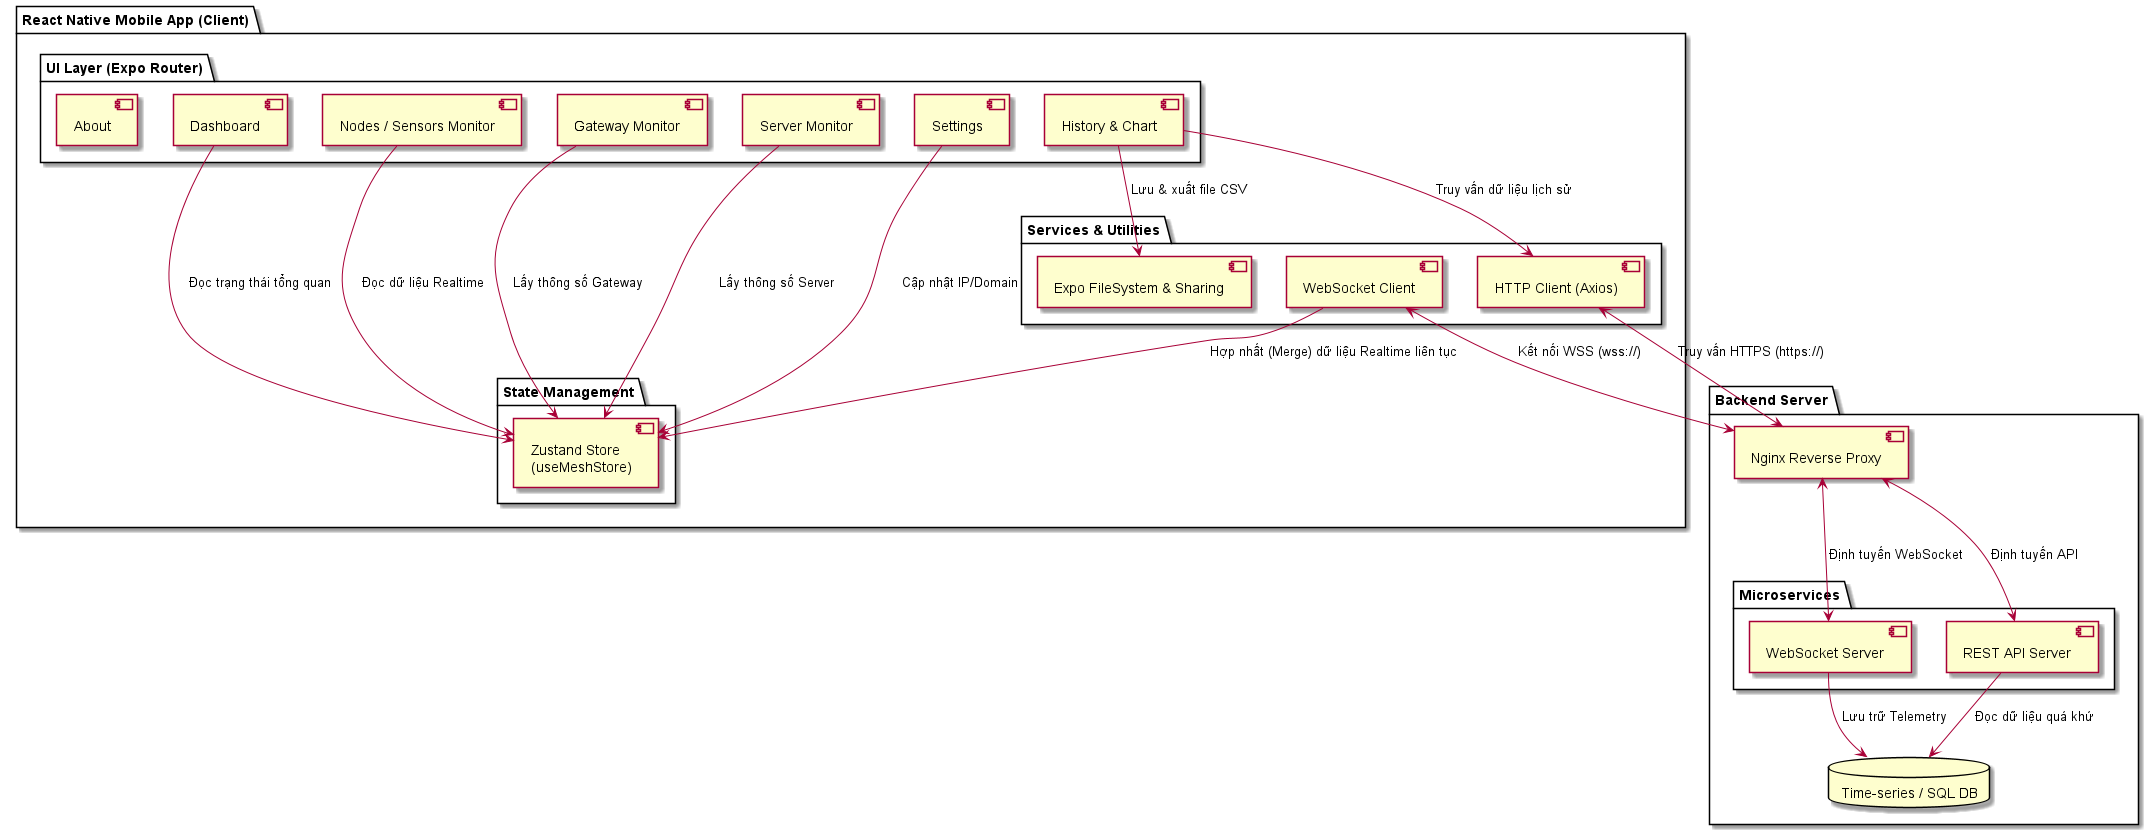
\includegraphics[width=\textwidth]{pic/app_architecture.png}
    \caption{Sơ đồ kiến trúc và luồng dữ liệu tổng thể của ứng dụng}
\end{figure}

\textbf{Giải thích sơ đồ kiến trúc:}
\begin{itemize}
    \item \textbf{Phân lớp UI (React Native \& Expo Router):} Đây là tầng giao diện tiếp xúc trực tiếp với người dùng, bao gồm các màn hình chính (Dashboard, Nodes, Sensors, History, Gateway, Server Monitor, Settings, About). Tầng này chịu trách nhiệm hiển thị dữ liệu và nhận các tương tác điều khiển từ người dùng.
    \item \textbf{Tầng Quản lý trạng thái (Zustand Store):} Trái tim của hệ thống lưu trữ trạng thái (State). Store này đóng vai trò trung tâm lưu trữ toàn bộ dữ liệu Realtime (thông số cảm biến, cấu hình IP/Domain, trạng thái Online/Offline). Bằng cơ chế "State Merging", nó tự động hợp nhất hàng loạt gói tin đến từ WebSocket để đảm bảo giao diện (UI) chỉ cập nhật (Re-render) khi thực sự cần thiết, tối ưu hóa hiệu suất thiết bị di động.
    \item \textbf{Tầng Dịch vụ (Services \& Utilities):}
    \begin{itemize}
        \item \textit{WebSocket Client:} Thiết lập luồng truyền phát hai chiều siêu tốc để liên tục cập nhật telemetry từ các nút cảm biến.
        \item \textit{HTTP Client (Axios):} Chịu trách nhiệm thực hiện các lệnh gọi RESTful truyền thống để lấy dữ liệu quá khứ (History Data).
        \item \textit{Expo FileSystem:} Cung cấp khả năng truy xuất hệ thống tệp tin gốc của thiết bị (Native File System) để tạo và lưu tệp báo cáo dạng CSV.
    \end{itemize}
    \item \textbf{Luồng Backend Server \& Nginx:} Trên máy chủ thực tế, một Nginx Reverse Proxy sẽ đứng ra nhận toàn bộ lưu lượng (Traffic) từ App qua Port 443. Sau đó, nó tự động phân giải chứng chỉ bảo mật và chuyển tiếp (Routing) yêu cầu WebSockets vào vi dịch vụ WebSocket Server, và REST API vào HTTP Server. Dữ liệu cuối cùng được ghi xuống và truy xuất từ hệ thống cơ sở dữ liệu.
\end{itemize}

\subsection{Sơ đồ tuần tự các luồng chức năng chính}
Chuỗi tương tác của hệ thống được chia làm 4 luồng nghiệp vụ cơ bản, mỗi luồng đảm nhiệm một vai trò độc lập nhằm tối ưu hóa hiệu năng và khả năng bảo trì.

\subsubsection{Luồng Khởi tạo kết nối (Init \& Connect)}
\begin{figure}[H]
    \centering
    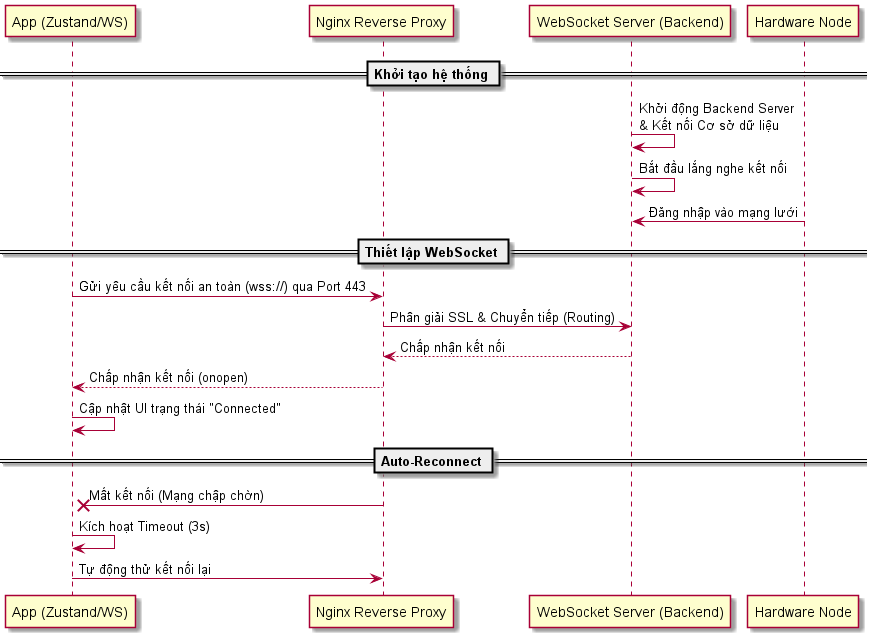
\includegraphics[width=\textwidth]{pic/seq_connect.png}
    \caption{Sơ đồ tuần tự Luồng khởi tạo kết nối.}
\end{figure}
Quá trình khởi tạo và thiết lập liên kết mạng lưới ban đầu được thực hiện theo các bước sau:
\begin{itemize}
    \item \textbf{Khởi động hệ thống:} Hệ thống Backend khởi động máy chủ WebSocket và thiết lập kết nối với hệ quản trị cơ sở dữ liệu. Sau đó, hệ thống liên tục lắng nghe và chờ đợi các thiết bị vi điều khiển (Node) truyền tải dữ liệu.
    \item \textbf{Thiết lập kết nối Client:} Ứng dụng di động (App) bắt đầu gửi yêu cầu kết nối an toàn thông qua giao thức WebSocket Secure (wss://) tới cổng 443 của Nginx Reverse Proxy. Nginx phân giải chứng chỉ bảo mật và chuyển tiếp (Routing) yêu cầu này tới máy chủ WebSocket của Backend (ws://). Backend chấp nhận kết nối và hai bên thiết lập đường truyền song công. Ứng dụng cập nhật trạng thái "Connected" trên giao diện.
    \item \textbf{Cơ chế tự phục hồi (Auto-Reconnect):} Trong thực tế công nghiệp, mạng Wi-Fi thường hay chập chờn. Khi có sự cố đứt kết nối mạng, ứng dụng sẽ phát hiện thông qua sự kiện ngắt kết nối. App sẽ đếm ngược (Timeout) 3 giây trước khi tự động gửi lại yêu cầu kết nối để đảm bảo giám sát không bị gián đoạn.
\end{itemize}


\subsubsection{Luồng Giám sát thời gian thực (Real-time telemetry)}
\begin{figure}[H]
    \centering
    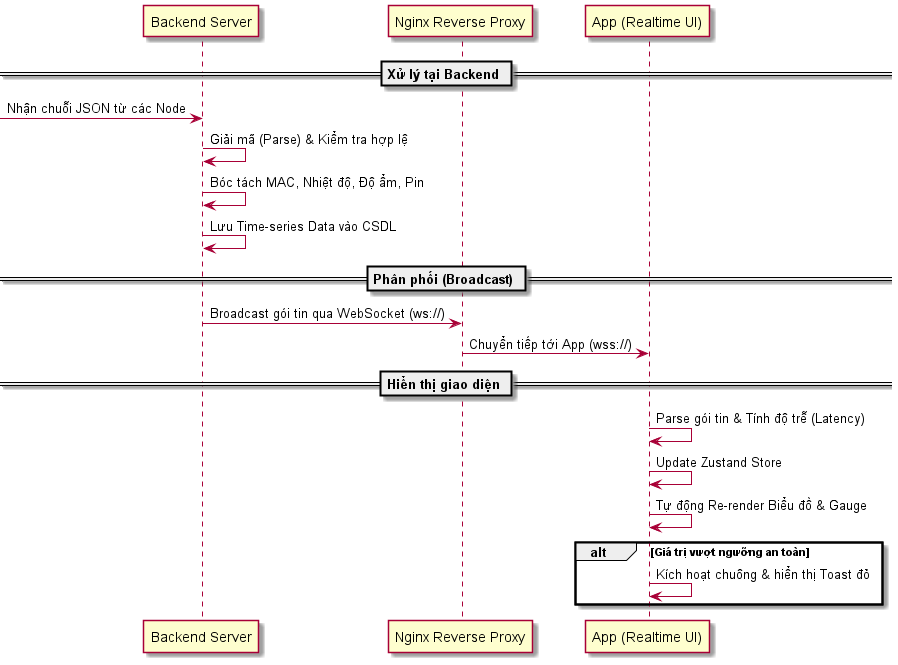
\includegraphics[width=\textwidth]{pic/puml_seq_realtime.png}
    \caption{Sơ đồ tuần tự Luồng giám sát thời gian thực.}
\end{figure}
Đây là luồng dữ liệu quan trọng nhất, đảm bảo tính tức thời của hệ thống giám sát:
\begin{itemize}
    \item \textbf{Xử lý tại Backend:} Hệ thống Backend đóng vai trò trung tâm tiếp nhận liên tục các chuỗi dữ liệu JSON gửi về từ các thiết bị phần cứng. Tại đây, Backend sẽ tiến hành giải mã (Parse), kiểm tra tính hợp lệ của gói tin, bóc tách các trường dữ liệu quan trọng (như MAC Address, Nhiệt độ, Độ ẩm, Trạng thái pin) và ngay lập tức lưu trữ vào hệ quản trị cơ sở dữ liệu. Quá trình lưu trữ này đảm bảo tính toàn vẹn của dữ liệu chuỗi thời gian (Time-series data), làm nền tảng cốt lõi phục vụ cho các tính năng truy vấn, xuất báo cáo và vẽ biểu đồ lịch sử sau này.
    \item \textbf{Phân phối (Broadcast):} Cùng lúc đó, Backend lập tức "đẩy" (Push) gói tin này tới Nginx để phân phối xuống tất cả các App đang kết nối qua kênh WebSocket an toàn (wss://).
    \item \textbf{Hiển thị giao diện:} App nhận gói tin và cập nhật thẳng vào bộ nhớ trạng thái trung tâm (Zustand Store). Các thành phần giao diện như Biểu đồ Sparkline, Đồng hồ đo (Gauge) sẽ tự động nhận diện và vẽ lại. Nếu giá trị cảm biến vượt ngưỡng an toàn cấu hình trước, một thông báo Toast màu đỏ kèm cảnh báo sẽ lập tức xuất hiện.
\end{itemize}


\subsubsection{Luồng Truy vấn dữ liệu lịch sử (History query)}
Chức năng này cho phép quản trị viên xem lại biến động dữ liệu môi trường trong quá khứ:
\begin{figure}[H]
    \centering
    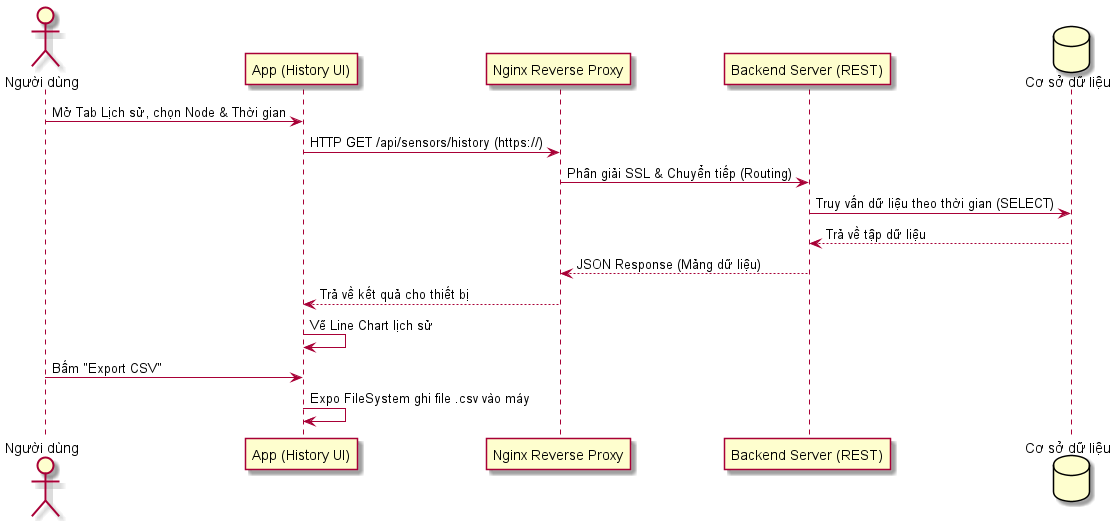
\includegraphics[width=\textwidth]{pic/puml_seq_history.png}
    \caption{Sơ đồ tuần tự Luồng truy vấn dữ liệu lịch sử.}
\end{figure}
\begin{itemize}
    \item \textbf{Truy vấn API:} Thay vì dùng WebSocket, luồng này sử dụng kiến trúc RESTful thông qua hai Endpoint chính:
    \begin{itemize}
        \item \texttt{GET /api/history/meta}: Lấy danh sách các MAC Address đã từng gửi dữ liệu để người dùng có thể chọn lọc.
        \item \texttt{GET /api/history/series}: Trích xuất dữ liệu chuỗi thời gian dựa trên các tham số gửi kèm (như \texttt{mac}, \texttt{from}, \texttt{to}, \texttt{limit}).
    \end{itemize}
    Khi người dùng thao tác trên Tab Lịch sử, ứng dụng sẽ gửi lệnh HTTP GET an toàn (https://) tới Nginx Reverse Proxy, sau đó Nginx chuyển tiếp yêu cầu này tới Backend Server.
    \item \textbf{Trích xuất cơ sở dữ liệu:} Backend nhận lệnh và thực thi câu truy vấn trích xuất dữ liệu với điều kiện thời gian tương ứng. Sau đó, hệ thống đóng gói tập hợp các bản ghi thành mảng JSON và trả về cho thiết bị thông qua Nginx.
    \item \textbf{Vẽ biểu đồ và Xuất file:} Ứng dụng tiến hành vẽ đường biểu đồ (Line chart). Đặc biệt, khi cần làm báo cáo, người dùng có thể bấm nút "Export CSV", hệ thống sẽ tận dụng thư viện Expo FileSystem để tạo ra một file \texttt{.csv} chuẩn và lưu thẳng vào điện thoại di động.
\end{itemize}

\subsubsection{Luồng Cập nhật phần mềm (FOTA)}
Quá trình cập nhật Firmware từ xa (Over-The-Air) giúp tiết kiệm đáng kể công sức bảo trì:
\begin{itemize}
    \item \textbf{Quản lý phiên bản:} Khi mở chức năng FOTA, App gửi lệnh HTTP GET để lấy danh sách các file firmware đuôi \texttt{.bin} đang được lưu sẵn trên Server Gateway.
    \item \textbf{Phát lệnh cập nhật:} Người quản trị chọn file tương ứng và gửi lệnh HTTP POST đẩy lệnh cập nhật xuống Gateway, nhắm tới một thiết bị cụ thể trong mạng lưới.
    \item \textbf{Truyền dữ liệu không dây:} Gateway báo hiệu cho Node. Khi Node sẵn sàng nhận, Gateway chia nhỏ file \texttt{.bin} thành các khối dữ liệu (block) và truyền không dây xuống qua mạng Mesh. Node nhận, ghi đè thẳng vào phân vùng bộ nhớ Flash và tự khởi động lại.
\end{itemize}
\begin{figure}[H]
    \centering
    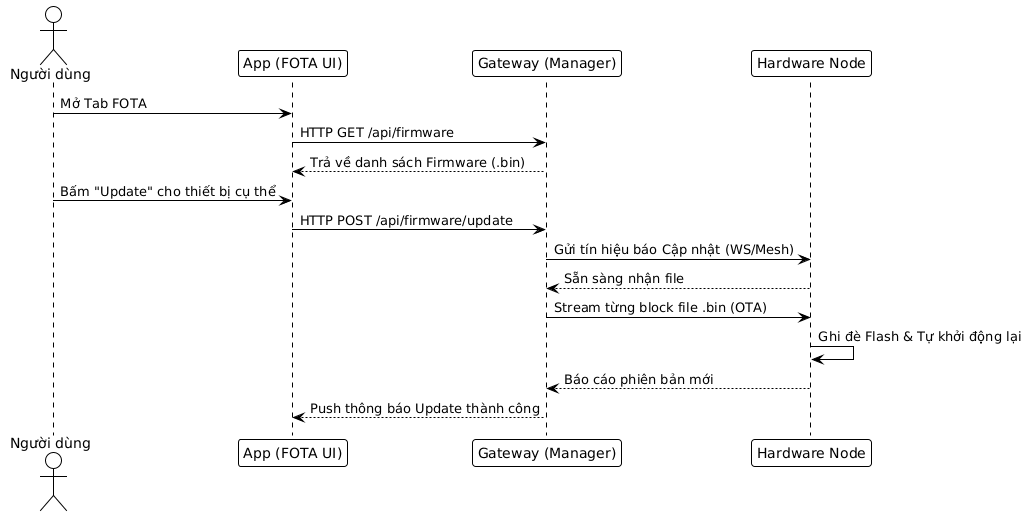
\includegraphics[width=\textwidth]{pic/puml_seq_fota.png}
    \caption{Sơ đồ tuần tự Luồng cập nhật phần mềm (FOTA).}
\end{figure}

\subsection{Cây thư mục chính trong mã nguồn src}
Để dễ dàng quản lý và mở rộng, mã nguồn dự án được tổ chức theo cấu trúc module hóa phân tách rõ ràng giữa Frontend và Backend. Sơ đồ dưới đây trình bày cấu trúc tổng thể của hệ thống:
\begin{figure}[H]
    \centering
    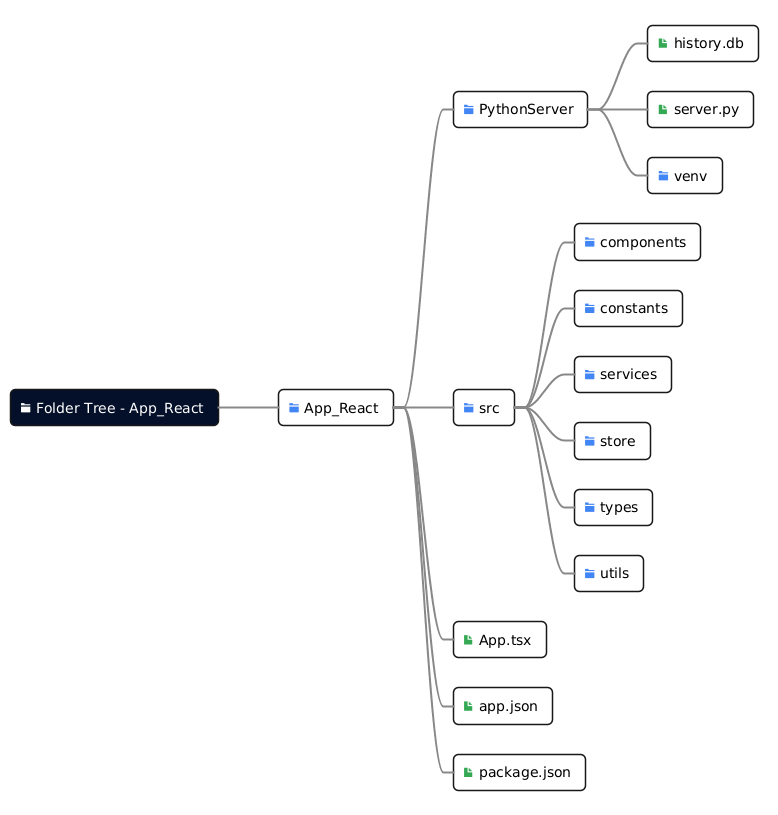
\includegraphics[width=\textwidth]{pic/puml_tree.png}
    \caption{Cấu trúc phân bổ thư mục tổng quan}
\end{figure}

Dưới đây là chi tiết phân rã các thư mục con bên trong thư mục \texttt{src} của ứng dụng React Native:

\subsubsection{Thư mục \texttt{components}}
Nơi chứa toàn bộ các UI component độc lập và có khả năng tái sử dụng cao trên toàn ứng dụng.
\begin{figure}[H]
    \centering
    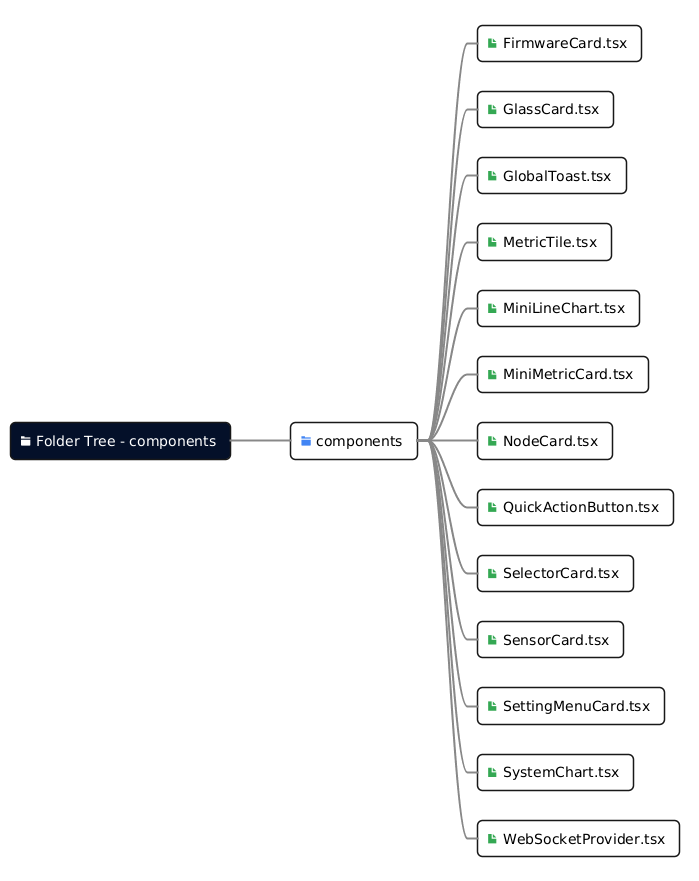
\includegraphics[width=\textwidth]{pic/puml_tree_components.png}
    \caption{Chi tiết các tập tin trong thư mục components}
\end{figure}
\begin{itemize}
    \item \textbf{FirmwareCard.tsx}: Giao diện thẻ quản lý cập nhật phần mềm từ xa (FOTA).
    \item \textbf{GlassCard.tsx}: Component tạo hiệu ứng nền kính mờ (Glassmorphism) dùng chung.
    \item \textbf{GlobalToast.tsx}: Thành phần hiển thị thông báo nổi (toast) toàn cục.
    \item \textbf{MetricTile.tsx, MiniMetricCard.tsx}: Các thẻ nhỏ gọn hiển thị chỉ số cảm biến (nhiệt độ, độ ẩm).
    \item \textbf{MiniLineChart.tsx, SystemChart.tsx}: Các thành phần vẽ biểu đồ theo dõi lịch sử dữ liệu trực quan.
    \item \textbf{NodeCard.tsx, SensorCard.tsx}: Giao diện hiển thị trạng thái và chi tiết dữ liệu của từng thiết bị trong mạng.
    \item \textbf{QuickActionButton.tsx}: Các nút thao tác nhanh (kết nối, làm mới).
    \item \textbf{SettingMenuCard.tsx, SelectorCard.tsx}: Giao diện cài đặt và tùy chọn thông số ngưỡng cảnh báo.
    \item \textbf{WebSocketProvider.tsx}: Cung cấp bối cảnh (Context) quản lý kết nối WebSocket thời gian thực cho toàn bộ ứng dụng.
\end{itemize}

\subsubsection{Thư mục \texttt{store}}
Sử dụng thư viện Zustand để quản lý State (trạng thái) toàn cục, giúp ứng dụng tự động cập nhật giao diện mà không cần truyền Props phức tạp.
\begin{figure}[H]
    \centering
    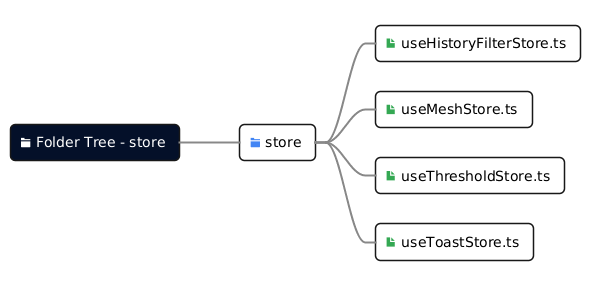
\includegraphics[width=\textwidth]{pic/puml_tree_store.png}
    \caption{Chi tiết các tập tin trong thư mục store}
\end{figure}
\begin{itemize}
    \item \textbf{useHistoryFilterStore.ts}: Lưu trữ trạng thái của bộ lọc thời gian và thông số khi xem biểu đồ lịch sử.
    \item \textbf{useMeshStore.ts}: Quản lý dữ liệu trung tâm của toàn mạng lưới (danh sách thiết bị online/offline, dữ liệu cảm biến mới nhất).
    \item \textbf{useThresholdStore.ts}: Lưu trữ cấu hình các ngưỡng cảnh báo nguy hiểm do người dùng cài đặt.
    \item \textbf{useToastStore.ts}: Quản lý hàng đợi các thông báo hiển thị trên màn hình.
\end{itemize}

\subsubsection{Thư mục \texttt{services}}
Chứa các logic xử lý nghiệp vụ, giao tiếp với máy chủ (API) và phân tích luồng dữ liệu thô.
\begin{figure}[H]
    \centering
    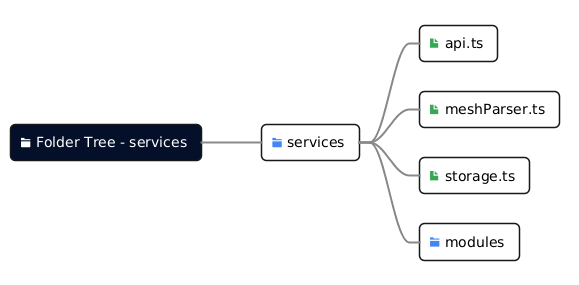
\includegraphics[width=\textwidth]{pic/puml_tree_services.png}
    \caption{Chi tiết các tập tin trong thư mục services}
\end{figure}
\begin{itemize}
    \item \textbf{api.ts}: Cung cấp các hàm gọi HTTP REST API giao tiếp với Backend (như lấy dữ liệu lịch sử).
    \item \textbf{meshParser.ts}: Đảm nhiệm logic phân tích cú pháp (parsing) các gói tin JSON thô nhận được từ Gateway thông qua WebSocket.
    \item \textbf{storage.ts}: Xử lý logic lưu trữ dữ liệu bền vững cục bộ trên thiết bị di động (sử dụng AsyncStorage).
\end{itemize}

\subsubsection{Các thư mục \texttt{constants}, \texttt{types}, \texttt{utils}}
Bao gồm các cấu hình màu sắc, hằng số tĩnh, các định nghĩa kiểu dữ liệu (TypeScript) và các hàm tiện ích hỗ trợ (format ngày tháng, số liệu).
\begin{figure}[H]
    \centering
    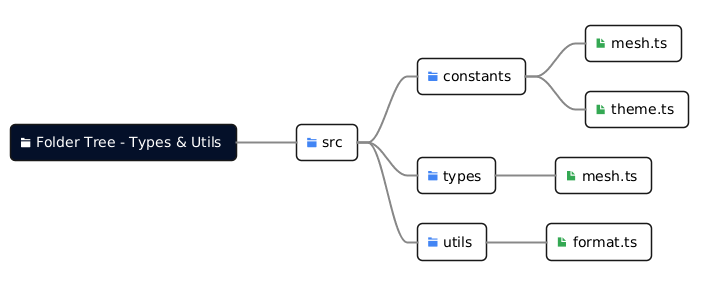
\includegraphics[width=0.8\textwidth]{pic/puml_tree_others.png}
    \caption{Chi tiết các tập tin cấu hình và tiện ích}
\end{figure}
\begin{itemize}
    \item \textbf{constants/mesh.ts, theme.ts}: Định nghĩa các hằng số không đổi của hệ thống và bộ quy chuẩn màu sắc, phông chữ (Theme) của UI.
    \item \textbf{types/mesh.ts}: Khai báo các Interface và Type bằng TypeScript để kiểm soát chặt chẽ cấu trúc dữ liệu của mạng Mesh.
    \item \textbf{utils/format.ts}: Chứa các hàm hỗ trợ định dạng chuỗi, ngày tháng, và làm tròn số liệu cảm biến.
\end{itemize}

\newpage

\section*{CHƯƠNG 3. DEMO THEO KỊCH BẢN}
\addcontentsline{toc}{section}{\numberline{}CHƯƠNG 3. DEMO THEO KỊCH BẢN}
\setcounter{section}{3}
\setcounter{subsection}{0}


\subsection{Kết quả Giao diện Ứng dụng Di động}
Ứng dụng được thiết kế theo phong cách hiện đại (Glassmorphism) với giao diện Dark Mode tối ưu cho việc giám sát thời gian thực. Dưới đây là các màn hình chức năng chính của ứng dụng.

\vspace{0.3cm}
\noindent\textbf{Video Demo Hệ thống:} \href{https://youtu.be/link-video-demo-cua-ban}{\underline{Nhấn vào đây để xem video minh họa toàn bộ hoạt động thực tế}}
\vspace{0.3cm}

\begin{figure}[H]
    \centering
    \begin{minipage}{0.45\textwidth}
        \centering
        \includegraphics[width=\linewidth]{pic/Dashboard_Menu.jpg}
        \caption{Giao diện Dashboard tổng quan}
    \end{minipage}\hfill
    \begin{minipage}{0.45\textwidth}
        \centering
        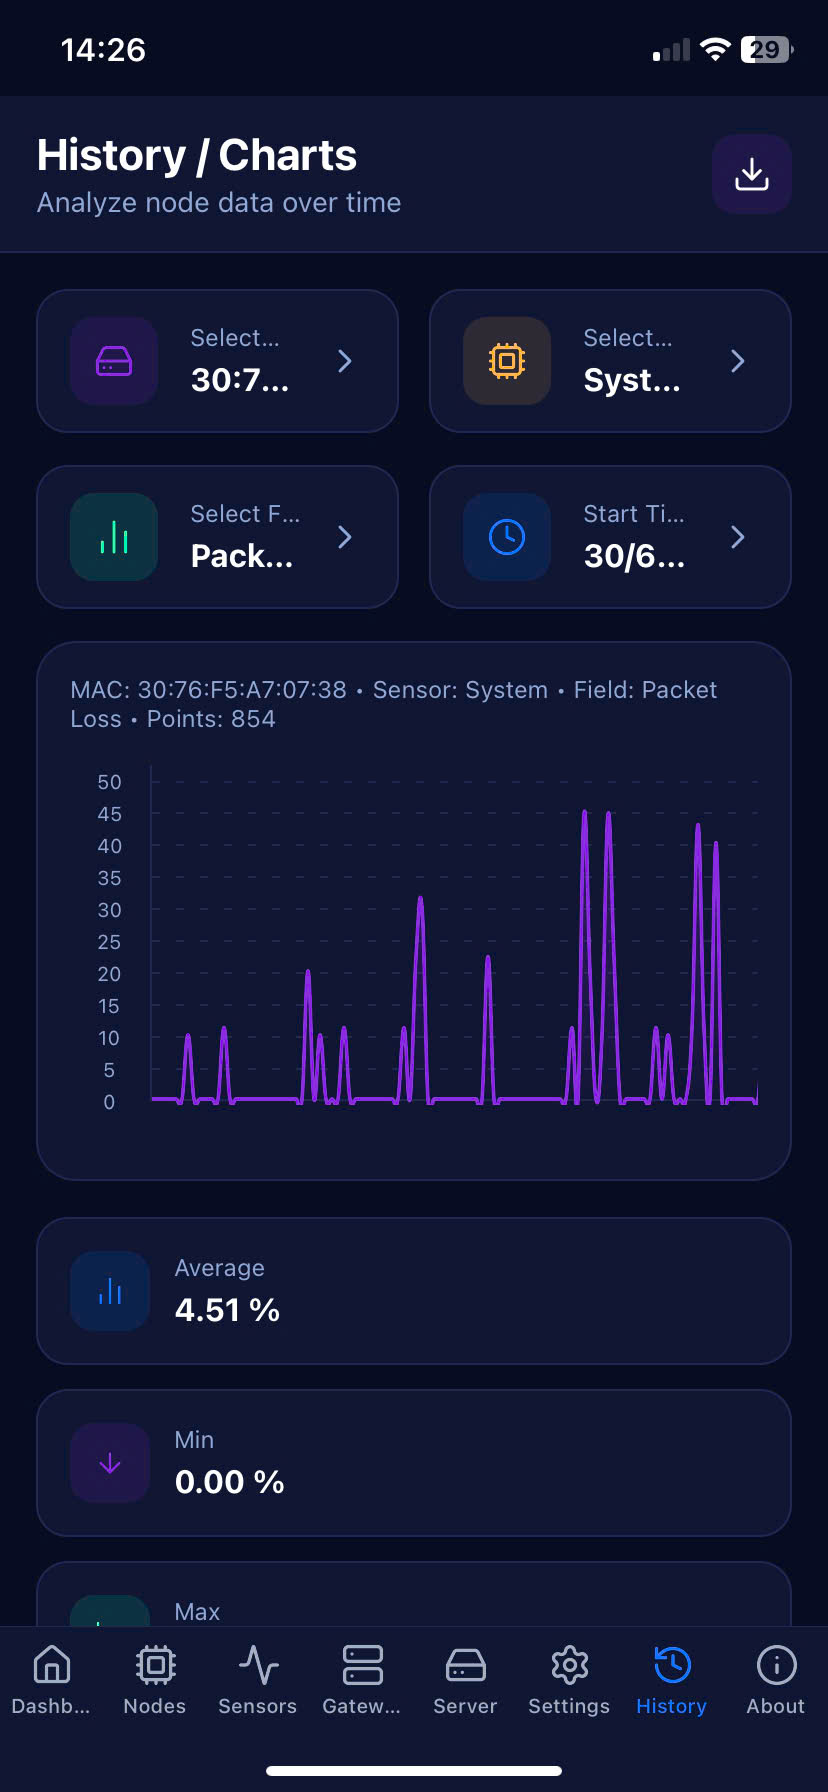
\includegraphics[width=\linewidth]{pic/History_Menu.jpg}
        \caption{Giao diện Lịch sử dữ liệu \& Biểu đồ}
    \end{minipage}
\end{figure}

Giao diện Dashboard đóng vai trò trung tâm, hiển thị trực quan thông số Nhiệt độ, Độ ẩm thông qua biểu đồ Sparkline và Gauge. Giao diện Lịch sử hỗ trợ truy vấn dữ liệu quá khứ, trực quan hóa bằng Line Chart và hỗ trợ tính năng xuất báo cáo (Export CSV).

\begin{figure}[H]
    \centering
    \begin{minipage}{0.45\textwidth}
        \centering
        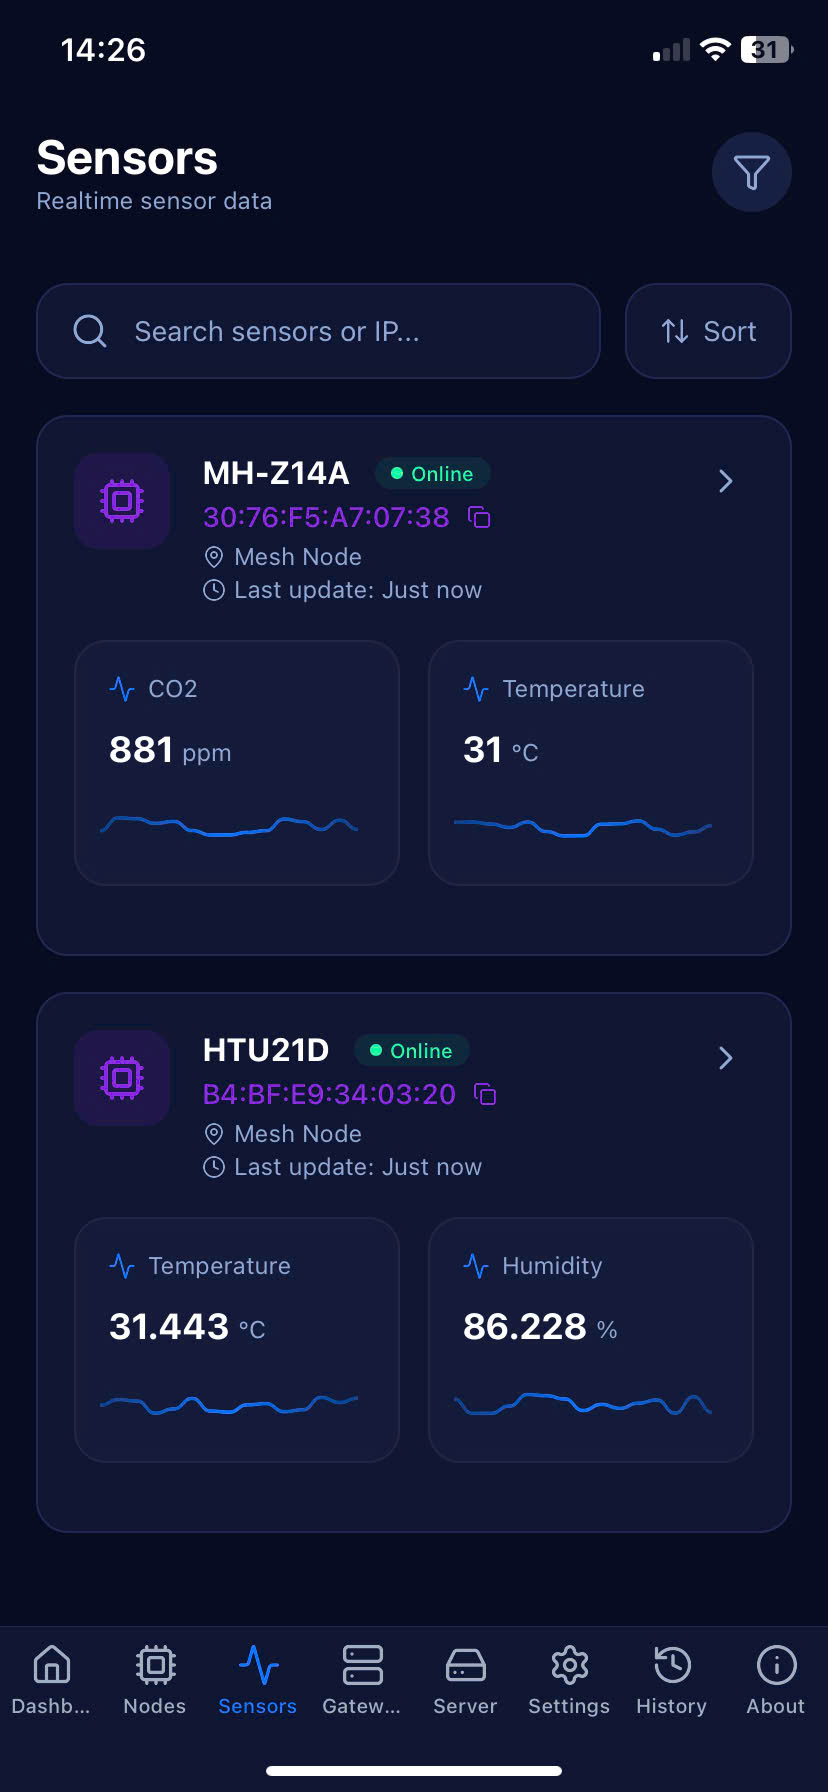
\includegraphics[width=\linewidth]{pic/Sensor_Menu.jpg}
        \caption{Quản lý danh sách Cảm biến (Nodes)}
    \end{minipage}\hfill
    \begin{minipage}{0.45\textwidth}
        \centering
        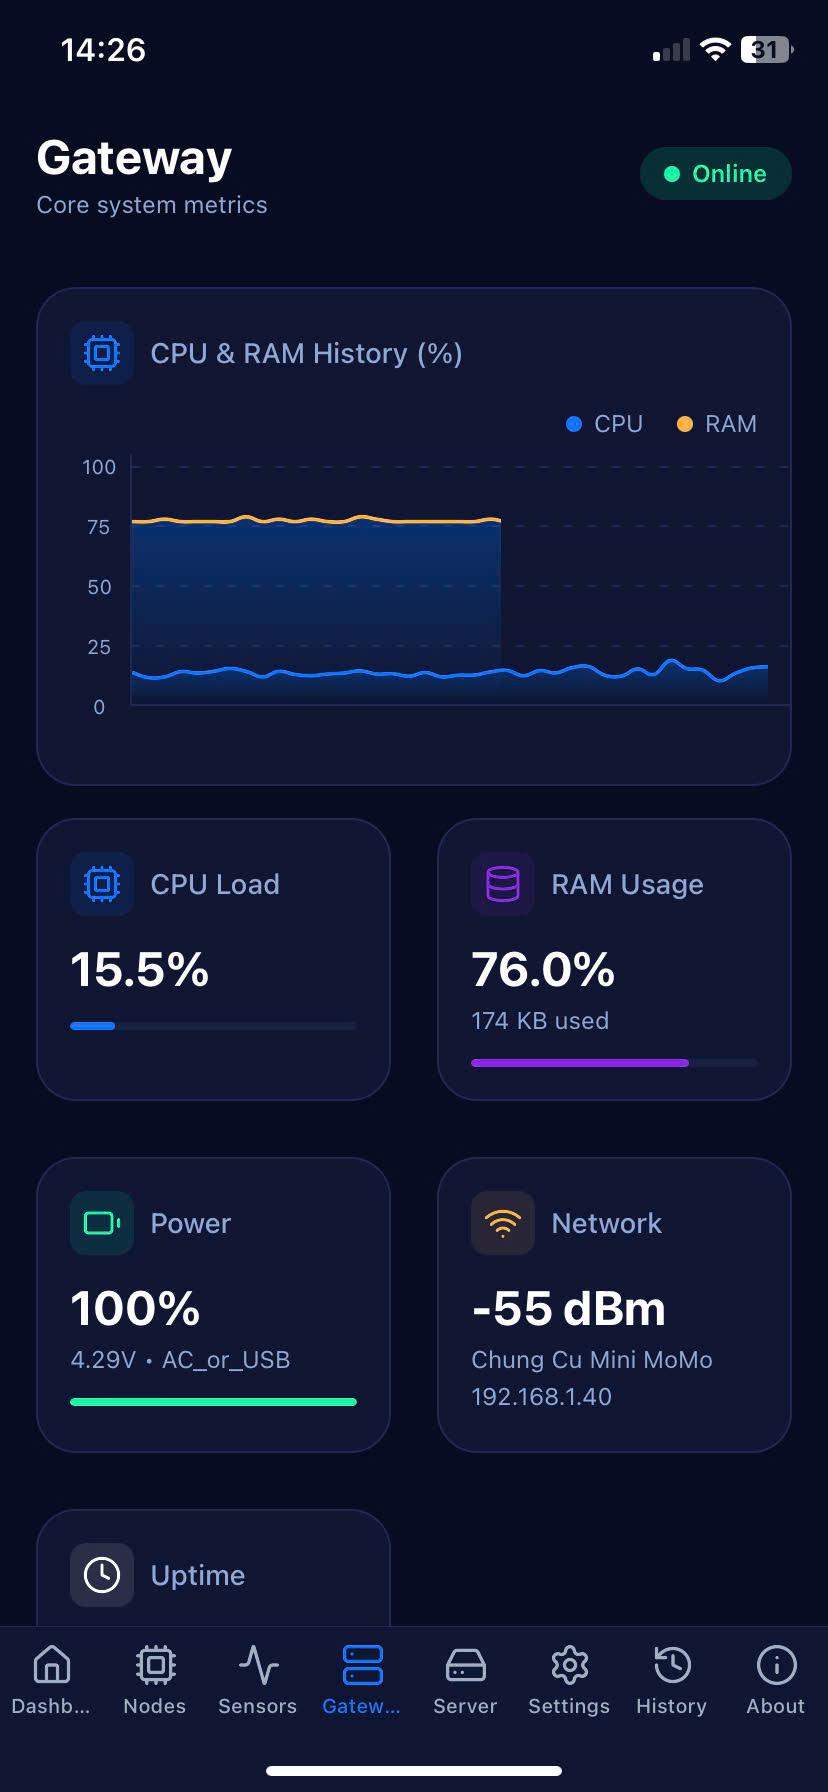
\includegraphics[width=\linewidth]{pic/Gateway_Menu.jpg}
        \caption{Quản lý danh sách Gateway}
    \end{minipage}
\end{figure}

Giao diện Cảm biến và Gateway giúp người quản trị dễ dàng theo dõi danh sách và trạng thái hoạt động (Online/Offline) của từng thiết bị phần cứng trong mạng lưới Mesh.

\begin{figure}[H]
    \centering
    \begin{minipage}{0.45\textwidth}
        \centering
        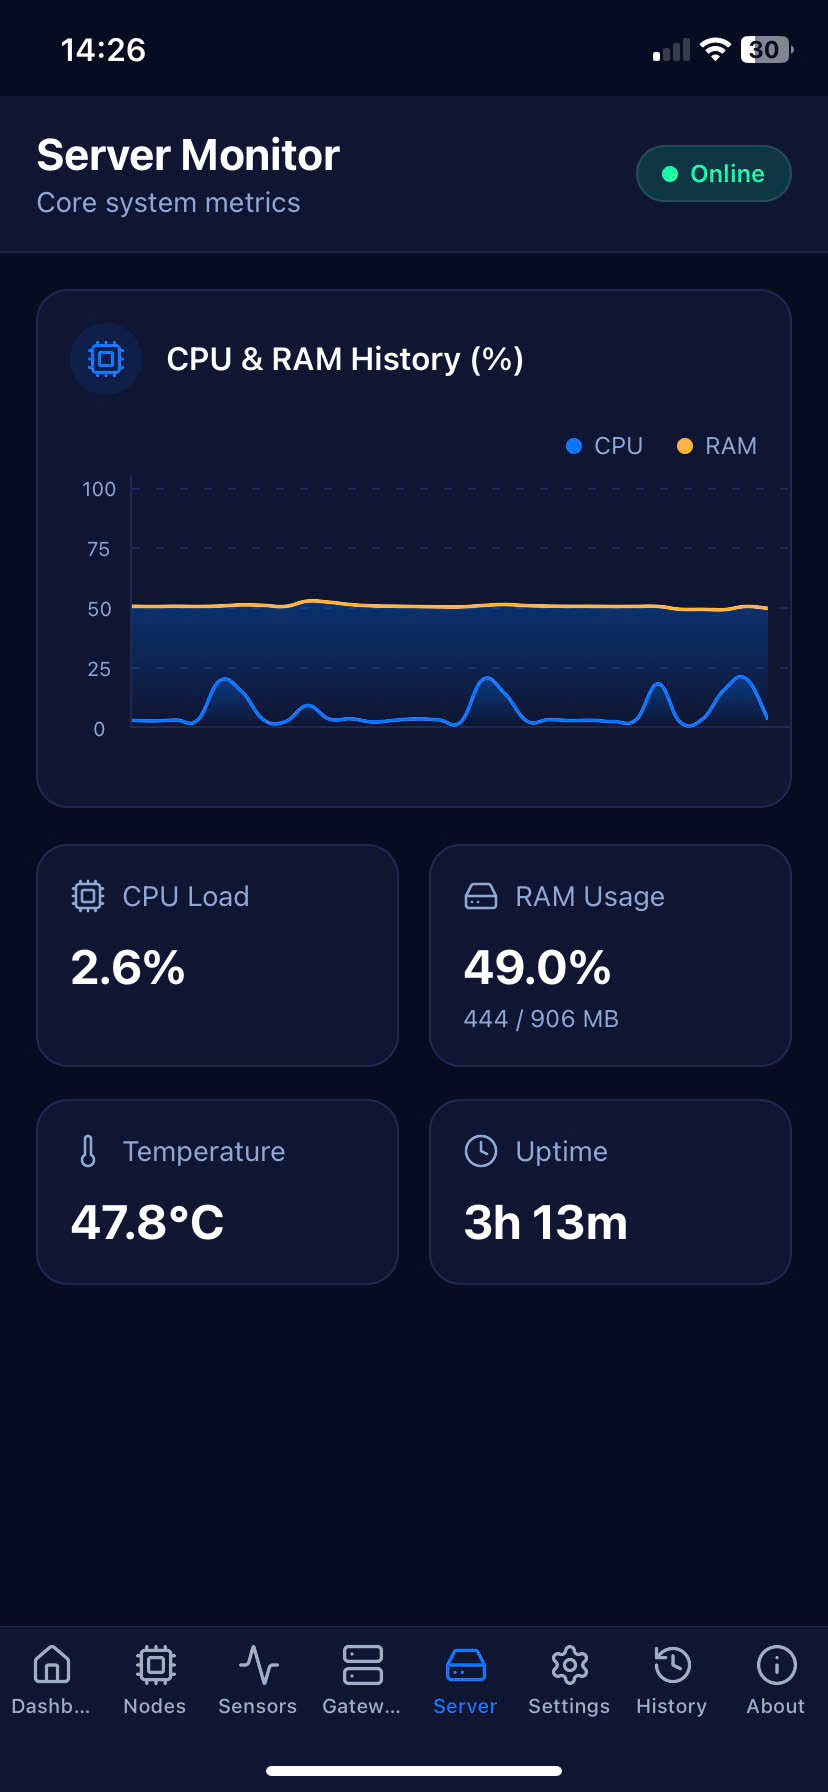
\includegraphics[width=\linewidth]{pic/Server_Menu.jpg}
        \caption{Giám sát Máy chủ (Server Health)}
    \end{minipage}\hfill
    \begin{minipage}{0.45\textwidth}
        \centering
        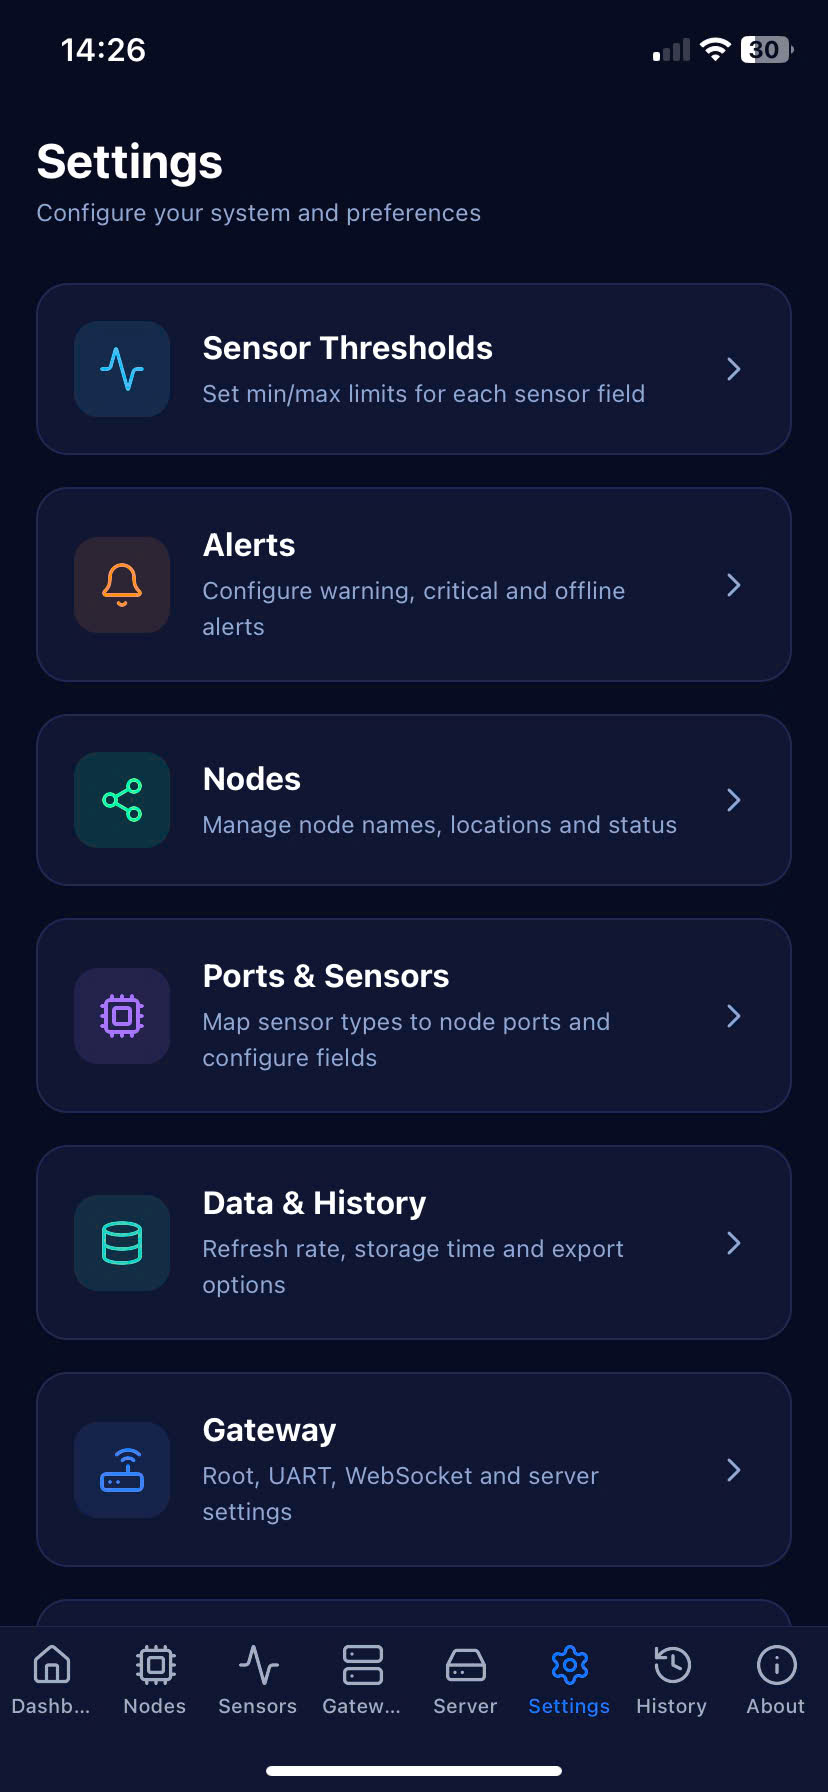
\includegraphics[width=\linewidth]{pic/Setting_Menu.jpg}
        \caption{Giao diện Cài đặt (Settings)}
    \end{minipage}
\end{figure}

Menu Server cho phép quản trị viên xem nhanh tình trạng kết nối và sức khỏe của hệ thống Backend. Trong khi đó, màn hình Cài đặt cung cấp nơi thay đổi Endpoint API và cấu hình giao thức truyền tải của toàn bộ ứng dụng.

\begin{figure}[H]
    \centering
    \begin{minipage}{0.45\textwidth}
        \centering
        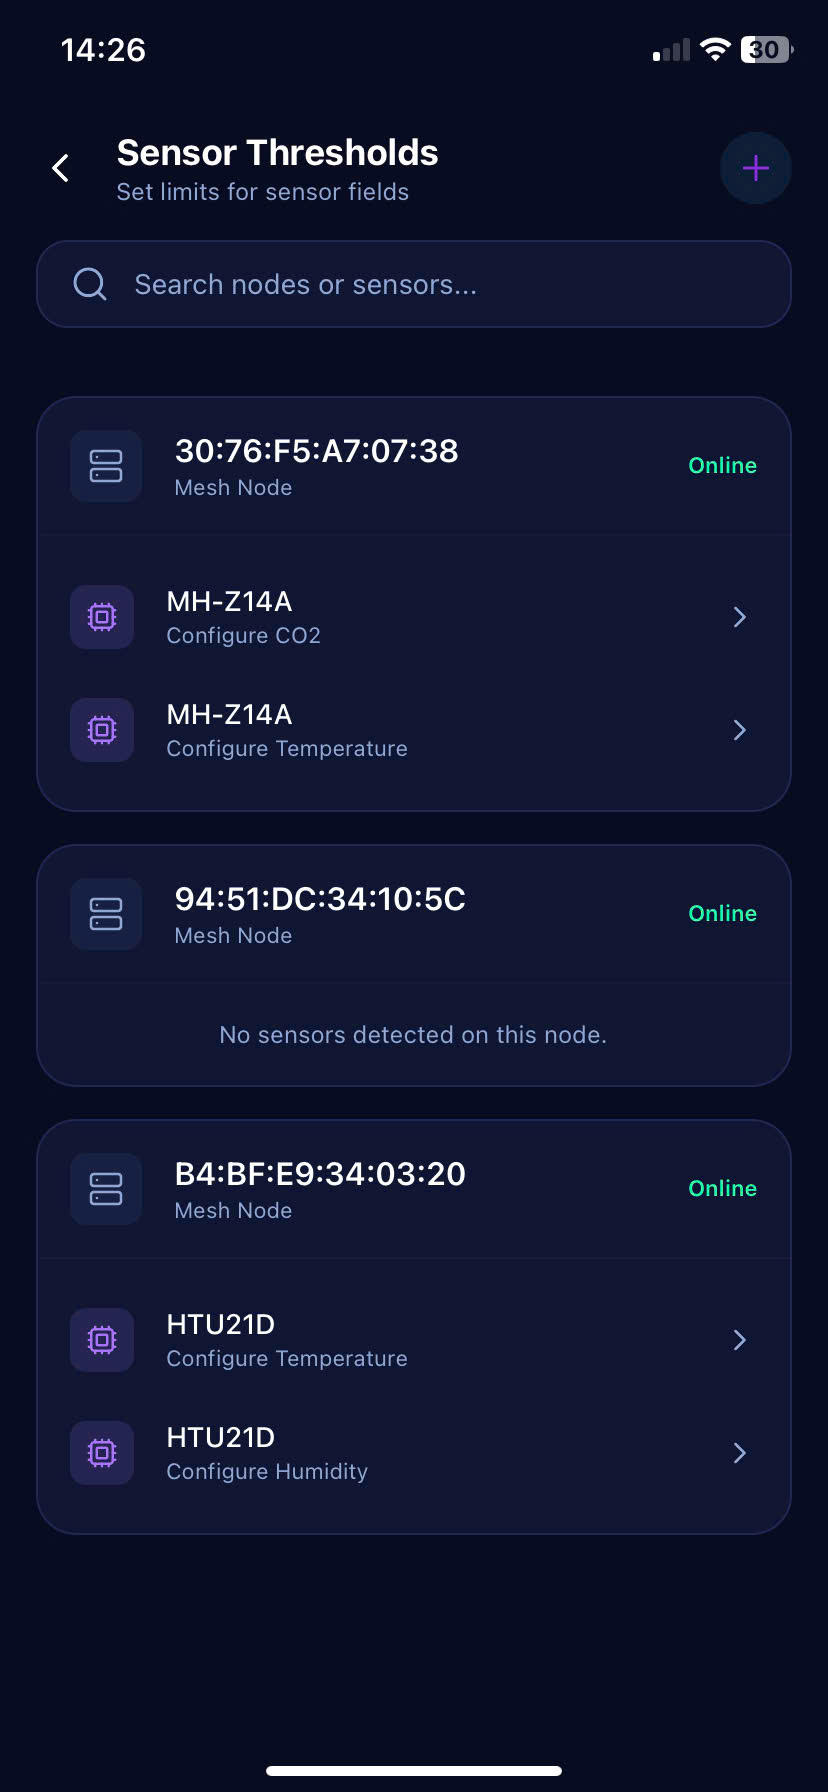
\includegraphics[width=\linewidth]{pic/SensorThreshold_Menu.jpg}
        \caption{Thiết lập ngưỡng cảnh báo}
    \end{minipage}\hfill
    \begin{minipage}{0.45\textwidth}
        \centering
        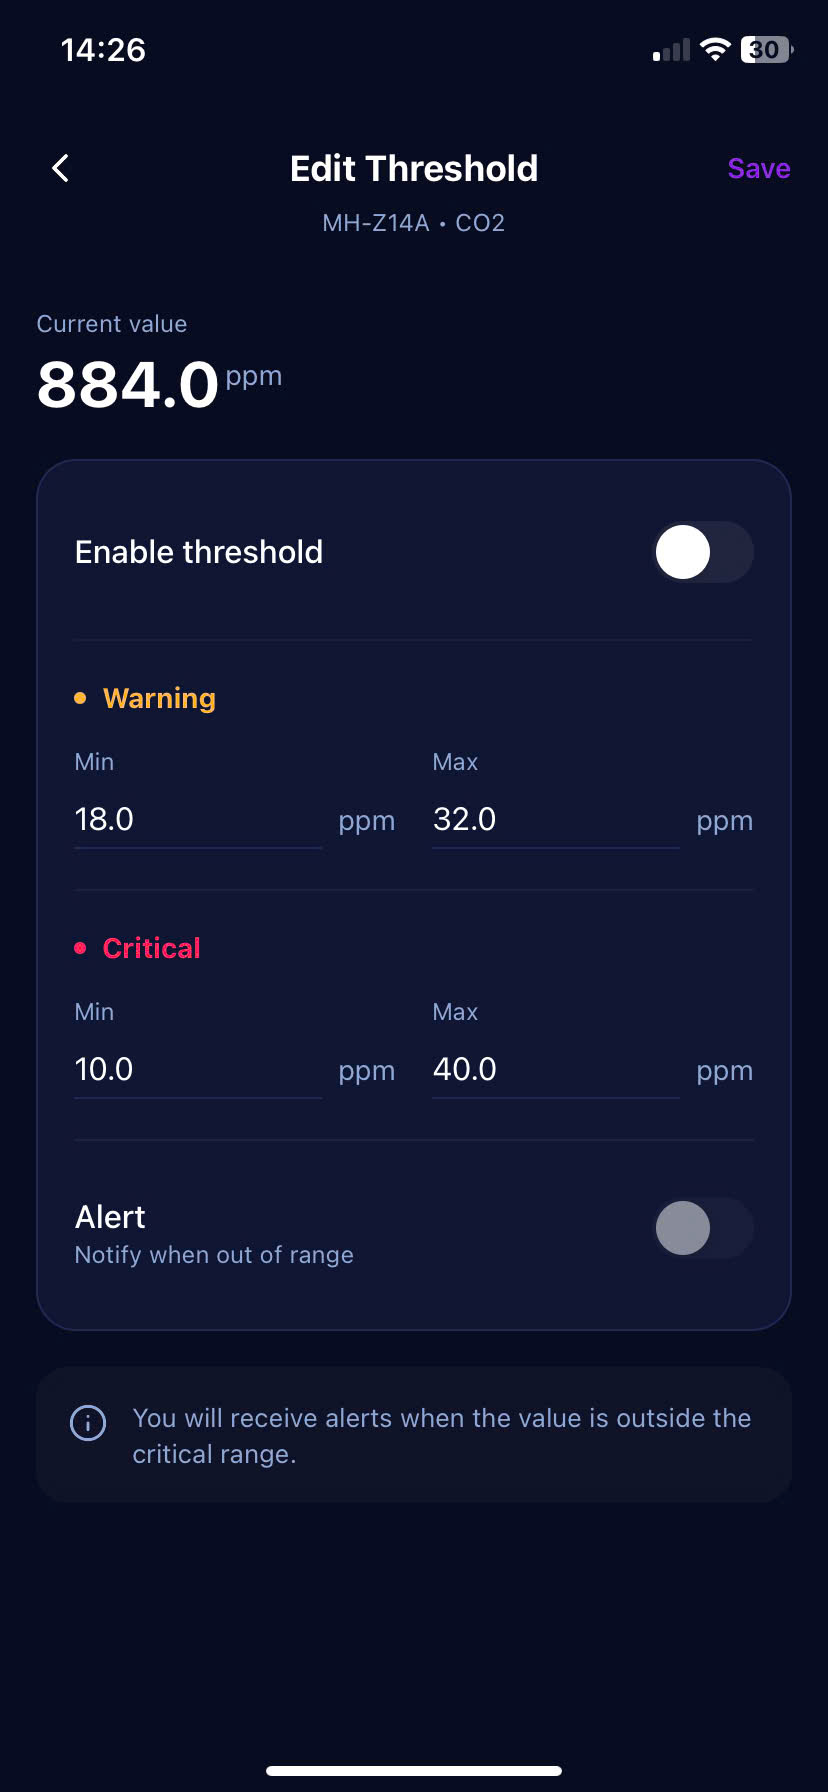
\includegraphics[width=\linewidth]{pic/EditSensor_Menu.jpg}
        \caption{Cập nhật thông tin Cảm biến}
    \end{minipage}
\end{figure}

Người dùng có thể cá nhân hóa mức cảnh báo nguy hiểm (Nhiệt độ tối đa, Độ ẩm tối thiểu...) tại màn hình Threshold. Ngoài ra, tính năng Edit Sensor hỗ trợ trực tiếp các thao tác cập nhật thông tin (CRUD) thiết bị lên cơ sở dữ liệu.

\begin{figure}[H]
    \centering
    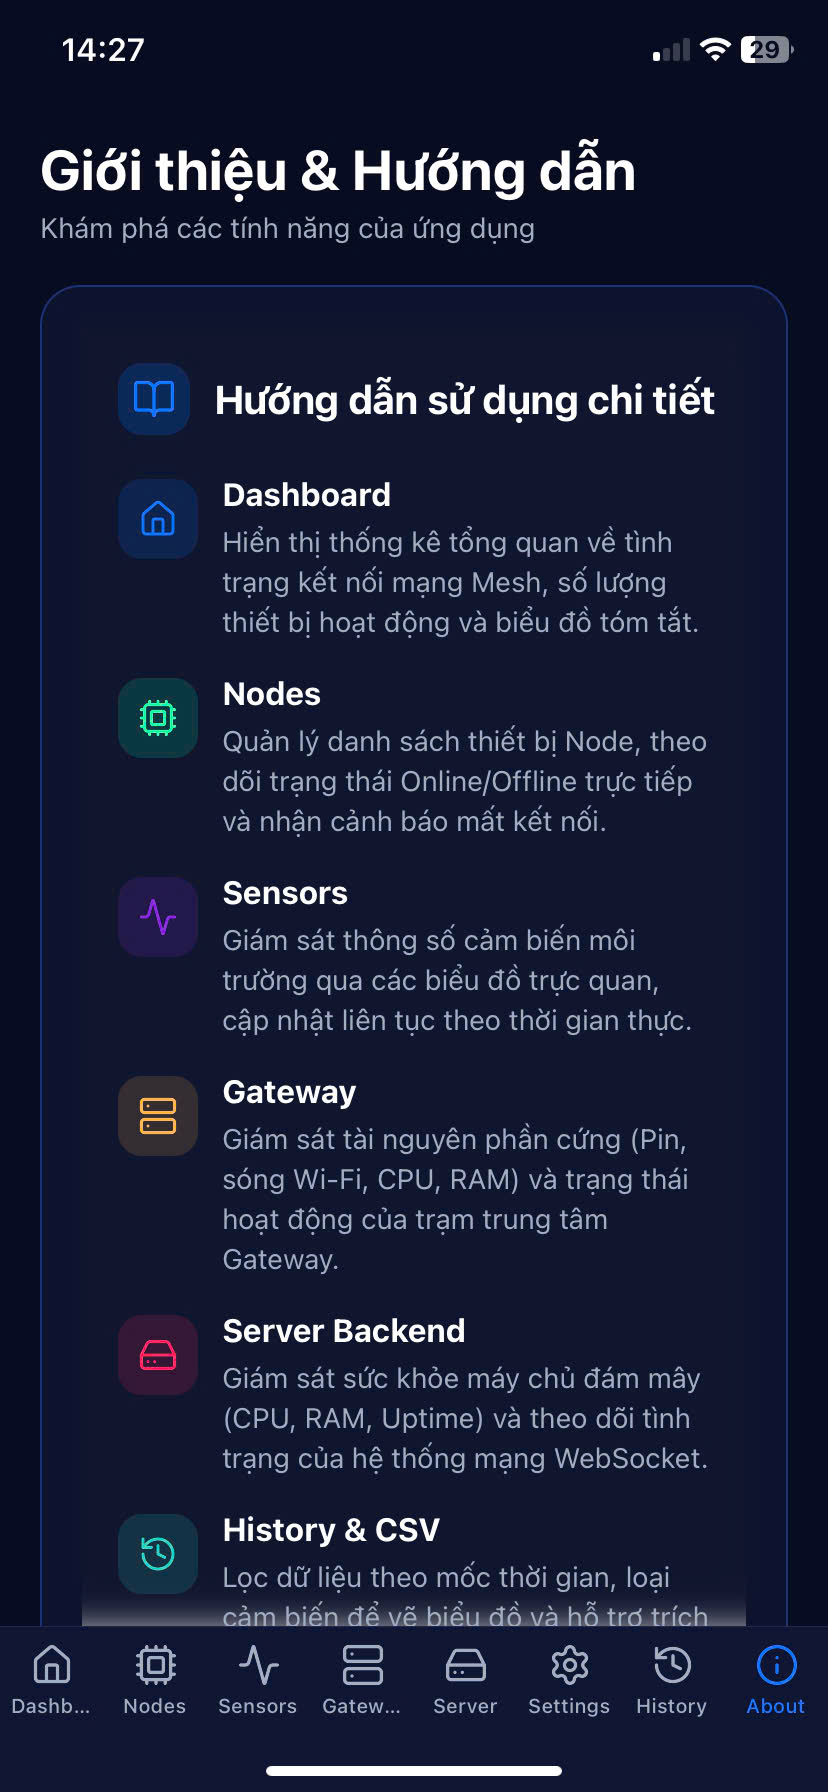
\includegraphics[width=0.45\textwidth]{pic/About_Menu.jpg}
    \caption{Trang thông tin \& Hướng dẫn (About)}
\end{figure}
Trang About tổng hợp tài liệu hướng dẫn sử dụng nhanh hệ thống, đồng thời hiển thị chi tiết thông tin, vai trò của từng thành viên trong nhóm phát triển dự án.

\subsection{Bảng tổng kết chức năng}
Bảng dưới đây tóm lược các chức năng cốt lõi của hệ thống đã được thực nghiệm và xác nhận thông qua kịch bản demo:

\begin{table}[H]
    \centering
    \renewcommand{\arraystretch}{1.3}
    \begin{tabularx}{\textwidth}{|l|>{\raggedright\arraybackslash}p{2.5cm}|X|>{\raggedright\arraybackslash}p{2.2cm}|c|}
        \hline
        \textbf{Menu/Phần} & \textbf{Chức năng} & \textbf{Mô tả chi tiết} & \textbf{Phụ trách} & \textbf{Tiến độ} \\
        \hline
        Dashboard & Thống kê tổng quan & Hiển thị tóm tắt tình trạng kết nối mạng Mesh và thông số nổi bật nhất của hệ thống. & H. Xuân Phú & 100\% \\
        \hline
        Nodes & Quản lý thiết bị & Liệt kê danh sách Node, theo dõi trạng thái Online/Offline trực tiếp và cảnh báo mất kết nối. & H. Quang Quân & 100\% \\
        \hline
        Sensors & Giám sát Realtime & Biểu đồ trực quan và danh sách thông số cảm biến môi trường cập nhật theo thời gian thực. & H. Quang Quân & 100\% \\
        \hline
        Server & Monitor Backend & Giám sát tài nguyên máy chủ (CPU, RAM, Uptime) và trạng thái hệ thống WebSocket. & H. Xuân Phú & 100\% \\
        \hline
        Gateway & Monitor Gateway & Giám sát tài nguyên phần cứng (CPU, RAM, Pin, Wi-Fi) và trạng thái của trạm trung tâm. & H. Quang Quân & 100\% \\
        \hline
        \multirow{2}{*}{History} & Truy vấn quá khứ & Lọc dữ liệu theo mốc thời gian, loại cảm biến, và vẽ biểu đồ lịch sử qua REST API. & H. Xuân Phú & 100\% \\ \cline{2-5}
        & Trích xuất CSV & Xử lý dữ liệu và tạo file báo cáo CSV cục bộ trên điện thoại để chia sẻ. & H. Xuân Phú & 100\% \\
        \hline
        Settings & Thiết lập Threshold & Tùy chỉnh các ngưỡng giới hạn (min/max) cảnh báo cho các thông số cảm biến. & H. Quang Quân & 100\% \\
        \hline
        About & Thông tin \& Hướng dẫn & Tích hợp hướng dẫn sử dụng và hiển thị thông tin dự án của nhóm. & H. Quang Quân & 100\% \\
        \hline
        Backend & Hạ tầng \& Máy chủ & Xây dựng HTTP REST API, cấu hình WebSockets và thiết lập Nginx Reverse Proxy trên máy chủ thực tế. & H. Xuân Phú & 100\% \\
        \hline
        Báo cáo & Tài liệu \& Slide & Soạn thảo báo cáo đồ án và slide thuyết trình tổng kết. & H. Xuân Phú, \par H. Quang Quân & 100\% \\
        \hline
    \end{tabularx}
    \caption{Bảng tổng kết chức năng hệ thống}
\end{table}

\newpage

\section*{CHƯƠNG 4. TỔNG KẾT}
\addcontentsline{toc}{section}{\numberline{}CHƯƠNG 4. TỔNG KẾT}
\setcounter{section}{4}
\setcounter{subsection}{0}

\subsection{Kết luận}
Dự án đã thiết kế và triển khai thành công một Hệ thống Giám sát Cảm biến Mạng Mesh hoàn chỉnh. Bằng việc kết hợp sức mạnh của React Native trên Frontend và kiến trúc bất đồng bộ của Python trên Backend, dự án mang lại một giao diện giám sát tốc độ cao, độ trễ thấp và khả năng mở rộng dễ dàng. Việc sử dụng công nghệ như Zustand, Expo, và WebSockets đã chứng minh tính hiệu quả vượt trội trong việc xử lý luồng dữ liệu thời gian thực cho hệ thống IoT.

\subsection{Hướng phát triển tương lai}
Mặc dù hệ thống đã đáp ứng tốt các yêu cầu đặt ra ở phạm vi mô hình, để triển khai thực tế trong môi trường công nghiệp quy mô lớn (Industrial IoT), nhóm phát triển đề xuất một số định hướng nâng cấp trong tương lai như sau:

\begin{itemize}
    \item \textbf{Nâng cấp hạ tầng giao tiếp với MQTT và Cloud:} 
    Thay thế chuẩn truyền thông WebSockets thuần bằng giao thức MQTT kết hợp với các nền tảng đám mây (AWS IoT Core, Firebase hoặc EMQX). Giải pháp này giúp tối ưu hóa băng thông, cải thiện độ ổn định và có khả năng chịu tải hàng ngàn thiết bị kết nối đồng thời.

    \item \textbf{Tích hợp Trí tuệ nhân tạo (AI/ML) vào phân tích dữ liệu:} 
    Triển khai các mô hình Học máy (Machine Learning) lên máy chủ Backend để phân tích sâu chuỗi dữ liệu thời gian thực. Cụ thể, hệ thống có thể dự đoán chu kỳ nhiệt độ, tối ưu hóa năng lượng cho thiết bị và phát hiện sớm các dị thường (Anomaly Detection) nhằm đưa ra cảnh báo trước khi sự cố xảy ra.

    \item \textbf{Hoàn thiện hệ thống Bảo mật và Phân quyền (Security \& IAM):} 
    Xây dựng module xác thực người dùng (Authentication) bằng JWT, kết hợp phân quyền quản trị đa cấp (Role-based Access Control). Đồng thời, triển khai cơ chế mã hóa đầu cuối (End-to-End Encryption) ở mức Payload cảm biến để đảm bảo tuyệt đối tính toàn vẹn của luồng dữ liệu truyền tải.
    
    \item \textbf{Mở rộng hệ sinh thái ứng dụng:} 
    Phát triển thêm phiên bản Web Admin Dashboard dùng chung API với Mobile App để quản trị viên có không gian thao tác trên màn hình lớn, đồng thời nâng cấp hệ thống báo cáo (Report) với các biểu đồ phân tích chuyên sâu.
\end{itemize}

\end{document}
